\documentclass[letterpaper,10pt]{article}

\usepackage{titling}
\usepackage{listings}
\usepackage{url}
\usepackage{setspace}
\usepackage{subfig}
\usepackage{sectsty}
\usepackage{pdfpages}
\usepackage{colortbl}
\usepackage{multirow}
\usepackage{relsize}
\usepackage{amsmath}
\usepackage{fancyvrb}
\usepackage{amsmath,amssymb,amsthm,graphicx,xspace}
\usepackage[titlenotnumbered,noend,noline]{algorithm2e}
\usepackage[compact]{titlesec}
\usepackage[default]{droidserif}
\usepackage[T1]{fontenc}
\usepackage{tikz}
\usetikzlibrary{arrows,automata,shapes,trees,matrix,chains,scopes,positioning,calc}
\tikzstyle{block} = [rectangle, draw, fill=blue!20, 
    text width=2.5em, text centered, rounded corners, minimum height=2em]
\tikzstyle{bw} = [rectangle, draw, fill=blue!20, 
    text width=4em, text centered, rounded corners, minimum height=2em]

\definecolor{namerow}{cmyk}{.40,.40,.40,.40}
\definecolor{namecol}{cmyk}{.40,.40,.40,.40}

\let\LaTeXtitle\title
\renewcommand{\title}[1]{\LaTeXtitle{\textsf{#1}}}


\newcommand{\handout}[5]{
  \noindent
  \begin{center}
  \framebox{
    \vbox{
      \hbox to 5.78in { {\bf ECE155: Engineering Design with Embedded Systems } \hfill #2 }
      \vspace{4mm}
      \hbox to 5.78in { {\Large \hfill #4  \hfill} }
      \vspace{2mm}
      \hbox to 5.78in { {\em #3 \hfill} }
    }
  }
  \end{center}
  \vspace*{4mm}
}

\newcommand{\lecture}[3]{\handout{#1}{#2}{#3}{Lecture #1}}
\newcommand{\tuple}[1]{\ensuremath{\left\langle #1 \right\rangle}\xspace}

\addtolength{\oddsidemargin}{-1.000in}
\addtolength{\evensidemargin}{-0.500in}
\addtolength{\textwidth}{2.0in}
\addtolength{\topmargin}{-1.000in}
\addtolength{\textheight}{1.75in}
\addtolength{\parskip}{\baselineskip}
\setlength{\parindent}{0in}
\renewcommand{\baselinestretch}{1.5}
\newcommand{\term}{Spring 2014}

\singlespace


\begin{document}

\lecture{ 14 --- UML}{\term}{Patrick Lam \& Jeff Zarnett}


\section*{Unified Modelling Language}
The \emph{Unified Modelling Language} (UML) is a language for
specifying and documenting the architecture of large object-oriented
software systems, using diagrams. UML version 2.2 includes 13
different diagrams, which can summarize a system's intended structure
(e.g. classes), behaviour, and interactions of components.

We are not going to examine all 13 diagrams since many of them are rather rarely used. We will focus on some of the most important ones.

\begin{center}
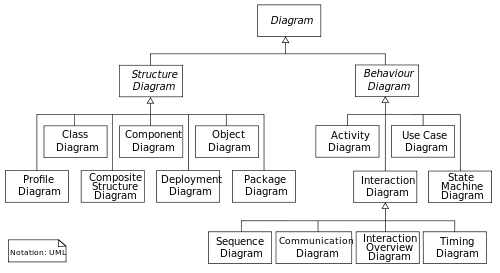
\includegraphics[width=0.5\textwidth]{images/uml-overview}
\end{center}

How much UML is used in industry will depend a lot on where you work. Some companies require it; others forbid it. Nevertheless, it is considered a common way to describe software and we need to learn it to be able to communicate with other programmers.

\paragraph{Historical Note.} UML combines earlier modelling languages,
and was initially developed by Grady Booch, James Rumbaugh, and Ivar
Jacobson (The Three Amigos) in the 1990s. Version 1.4.2 of UML is an ISO
standard, and future versions of UML are controlled by the Object
Management Group consortium.

UML has been developed since the late 1990s and is mostly, but not exclusively, for Object-Oriented Programming.

\paragraph{Resources.} There are a lot of webpages (some inaccurate)
with information about UML. Here are some resources:

\begin{itemize}
\item The official UML page is at \url{http://www.uml.org}; it contains 
links to the official specification, tutorials, and links to tool support.
\item One useful tutorial on practical UML is at \url{http://edn.embarcadero.com/article/31863}~\cite{uml:prac}. It contains sample diagrams, and also broken links.
\item The definitive UML book is:

$\qquad$ Grady Booch, James Rumbaugh, and Ivar Jacobson. \emph{Unified
Modeling Language User Guide,} 2nd Edition, Addison-Wesley, 2005.

\item Another book is 

$\qquad$ Dan Pilone and Neil Pitman. \emph{UML 2.0 in a Nutshell.} O'Reilly Media, 2005.

\item Official specification: \url{http://www.omg.org/technology/documents/formal/uml.htm}.
\end{itemize}


\paragraph{Benefits of UML.} We are teaching UML because it is a well-known
language for talking about software designs. In particular:

\begin{itemize}
\item UML is a visual language, and UML models are diagrams, so they're easy
to glance at.
\item UML models are largely self-documenting.
\item UML is agnostic in terms of software processes or development lifecycles.
\item UML is an open standard (not owned by any one company).
\item UML is good for object-oriented languages, which are quite common
in industry.
\end{itemize}

\paragraph{Criticisms of UML.} Here are a few complaints one might have:

\begin{itemize}
\item UML is all syntax, no meaning.
\item UML contains redundant and infrequently-used constructs.
\item UML is complex and difficult to learn.
\item UML only works for object-oriented languages.
\item UML tools don't play nicely together.
\end{itemize}

\paragraph{UML Diagrams.}
Let's look at the different categories of UML diagrams in UML 2.2:
\begin{itemize}
\item \emph{Structure Diagrams} represent the static application structure.

$\qquad$ Examples: class diagrams, object diagrams, component diagrams,
composite structure diagrams, package diagrams, deployment diagrams.

\item \emph{Behaviour Diagrams} encode the usage of components,
the activity of components, and finite-state machines summarizing components'
states.

$\qquad$ Examples: use case diagrams, activity diagrams, state machine diagrams.

\item \emph{Interaction Diagrams} describe how components interact;
  they may communicate or synchronize with each other, potentially
  respecting timing constraints.  

$\qquad$ Examples: sequence diagrams, communication diagrams, timing diagrams,
and interaction overview diagrams.
\end{itemize}

\paragraph{Tool Support.} A number of software tools can create UML diagrams,
including Microsoft Visio and {\tt dia}. Some tools can generate
source code from UML diagrams and UML diagrams from source code; if a
tool can do both, we say that it \emph{round-trips}. Tools can also,
to some extent, automatically generate test cases and test suites from
UML diagrams.

\section*{UML Class Diagrams}
The basic UML diagram is the class diagram, which describes the members of
a class. You saw this in ECE150, although maybe it wasn't called a class
diagram. Members include attributes/fields and operations (constructors,
destructors, methods, indexers, and properties).

Here's a simple example of a UML diagram.
\begin{center}
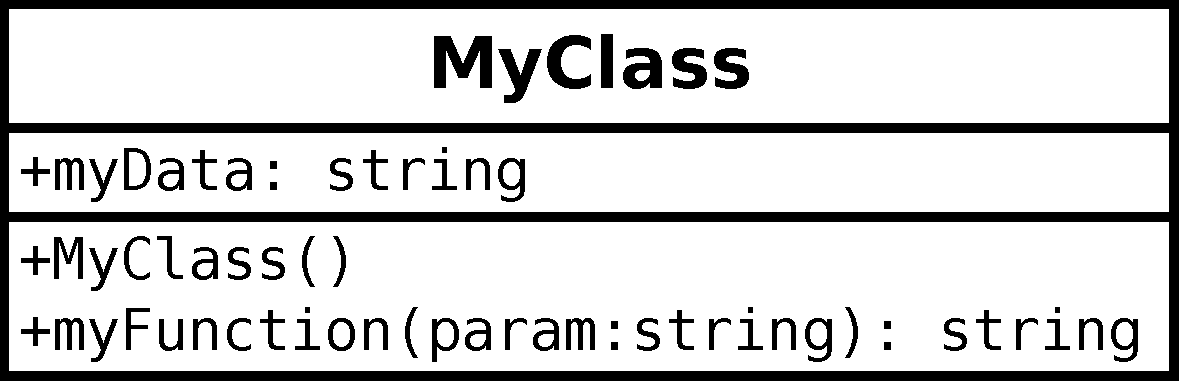
\includegraphics[width=.6\textwidth]{images/myclass.pdf}
\end{center}

\paragraph{UML Symbols.} Note that the above diagram includes a {\tt +}
for public visibility. Here are the possible visibility symbols:
\begin{itemize}
\item A {\tt +} (plus sign) indicates public visibility.
\item A {\tt -} (minus sign) indicates private visibility.
\item A {\tt \#} (hash sign) indicates protected visibility.
\end{itemize}

UML also uses the following symbols:
\begin{itemize}
\item A {\tt $\sim$} (tilde) indicates a destructor (in front of an operation) 
or package (as a visibility symbol).
\item An {\tt ..} (ellipsis) indicates a range of values.
\item A {\tt :} (colon) separates a name from a type.
\item A {\tt ,} (comma) separates items in a set.
\end{itemize}

\paragraph{More Complicated Example.} Here are some more features of UML:

\begin{center}
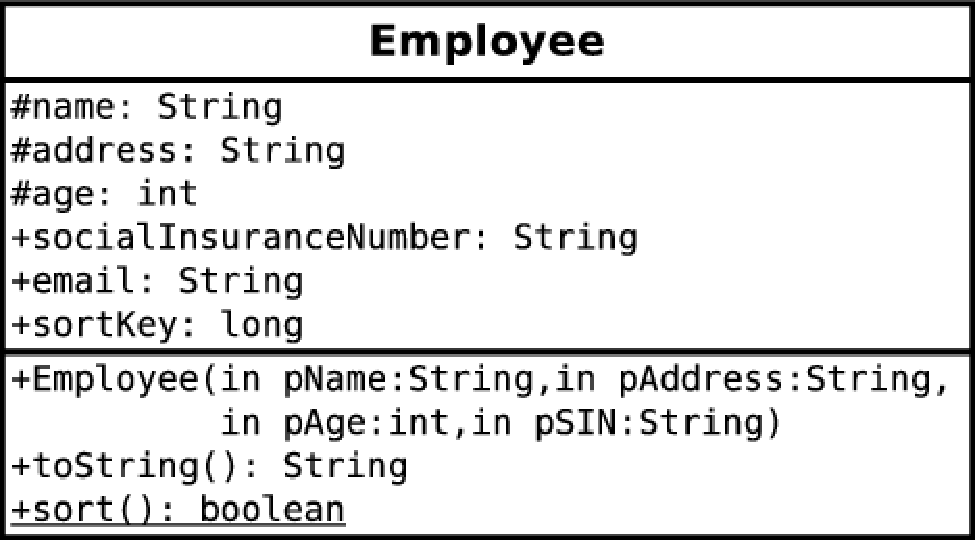
\includegraphics[height=8em]{images/Employee.pdf}
\end{center}

\begin{lstlisting}[language={Java},basicstyle=\small]
class Employee {
  protected String name;
  protected String address;
  protected int age;
  public String socialInsuranceNumber;
  public String email;
  public long sortKey;

  public Employee(String pName, String pAddress, int pAge, String pSIN) 
    { /* ... */ }
  @Override public String toString() { /* ... */ }
  public static boolean sort() { /* ... */ }
}
\end{lstlisting}

\subsection*{Class Hierarchies in UML}
UML includes a number of notations for representing relationships
between classes and instances.

The following relationships are between instances of classes.
\begin{itemize}
\item An \emph{association} represents a relationship between instances
of two classes.
\item An \emph{aggregation} is a type of association, typically between a
collection or container instance and its contents.
\item A \emph{composition} is another type of association, typically
used between a container and its contents. For a composition, the contents
don't make any sense if the container isn't around.
\end{itemize}

On the other hand, a \emph{generalization} relates base classes (not
instances) and their derived classes.

\paragraph{Associations.} There is an association between two classes
if there is a relationship between instances of the classes. This is
one of the ``has-a'' links between classes.  Typically one of the
classes can call methods on the other.
\begin{center}

\includegraphics[width=.5\textwidth]{images/association.pdf}
\end{center}
Instructors and courses are associated, but there is no subtype
relationship, and the types are not collection types. Instructors
teach between 0 and 3 courses per term. Each course has at least 1
instructor, but possibly an unlimited number. A method that the
instructor might call on the course might be {\tt giveLecture()}.

\paragraph{Aggregations and Compositions.} These specialized
types of associations also represent ``has-a'' relationships, but
more ``part-whole'' relationships.
\begin{center}
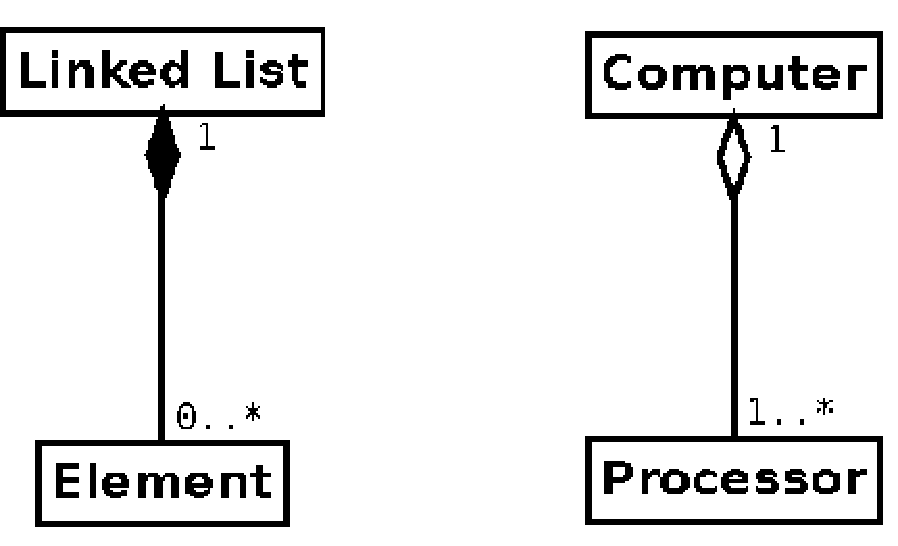
\includegraphics[height=7em]{images/aggr-comp.pdf}
\end{center}
A Linked List contains 0 or more Elements, but Elements belong to only
one Linked List; however, the composition means that we are
saying that Elements may not exist independently of a Linked List.

Computers contain 1 or more Processors, but Processors only
belong to 1 Computer. In an aggregation, we are stating that 
Processors can exist independently of a Computer.

\paragraph{Generalizations.} These relationships are between
classes.
\begin{center}
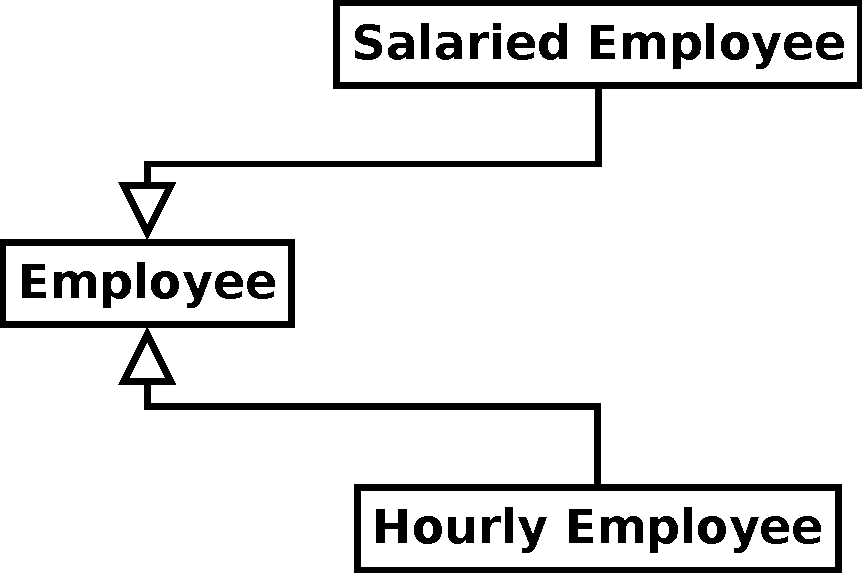
\includegraphics[width=.3\textwidth]{images/generalization.pdf}
\end{center}
Every Salaried Employee and Hourly Employee is an Employee, 
so Employees are generalizations of the Salaried and Hourly
Employee classes. In the code, you'd see that Salaried Employee
and Hourly Employee are subclasses of (``extend'') Employee.

\paragraph{Fancier UML Class Diagrams.} Here is a complex
UML class diagram:

\begin{center}
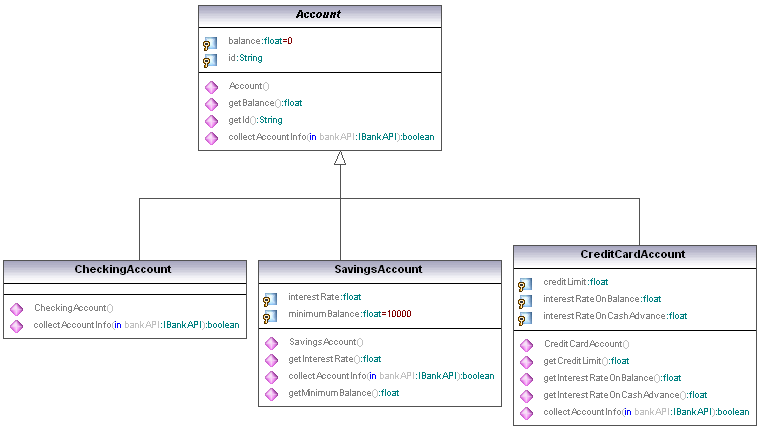
\includegraphics[width=\textwidth]{images/UML_class_diagram_example.png}
{\small \texttt{http://www.altova.com/umodel/class-diagrams.html}}
\end{center}
Note the member field initializations and the generalization link.


Here is another class diagram:
\begin{center}
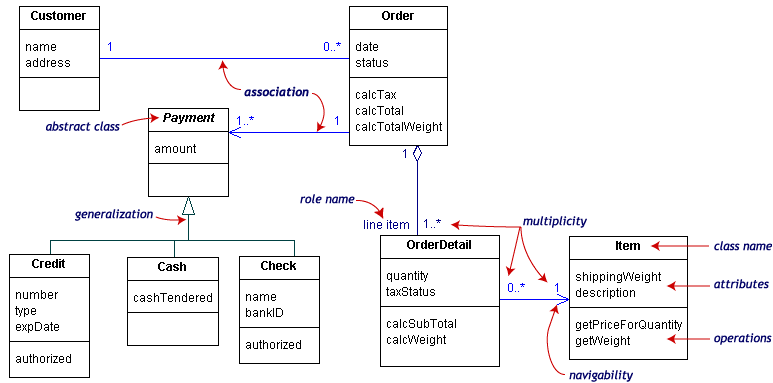
\includegraphics[width=\textwidth]{images/classdiagramno3d.png}
~\cite{uml:prac}
\end{center}

\section*{UML State Diagrams}
\paragraph{Goal.} You should be able to read a description of
a finite state machine (either in code or in text) and produce a
syntactically correct UML state diagram summarizing that design.

(The UML State Diagram examples are from \cite{UMLDistilled})

\subsection*{A Crash Course in Boxes and Lines}
You will be taught state diagrams in ECE~124, but not until much later in the term, and this cannot really afford to wait. So we shall begin with a short overview of state diagrams since they are needed to understand UML state diagrams. 

Here's an example.

\begin{center}
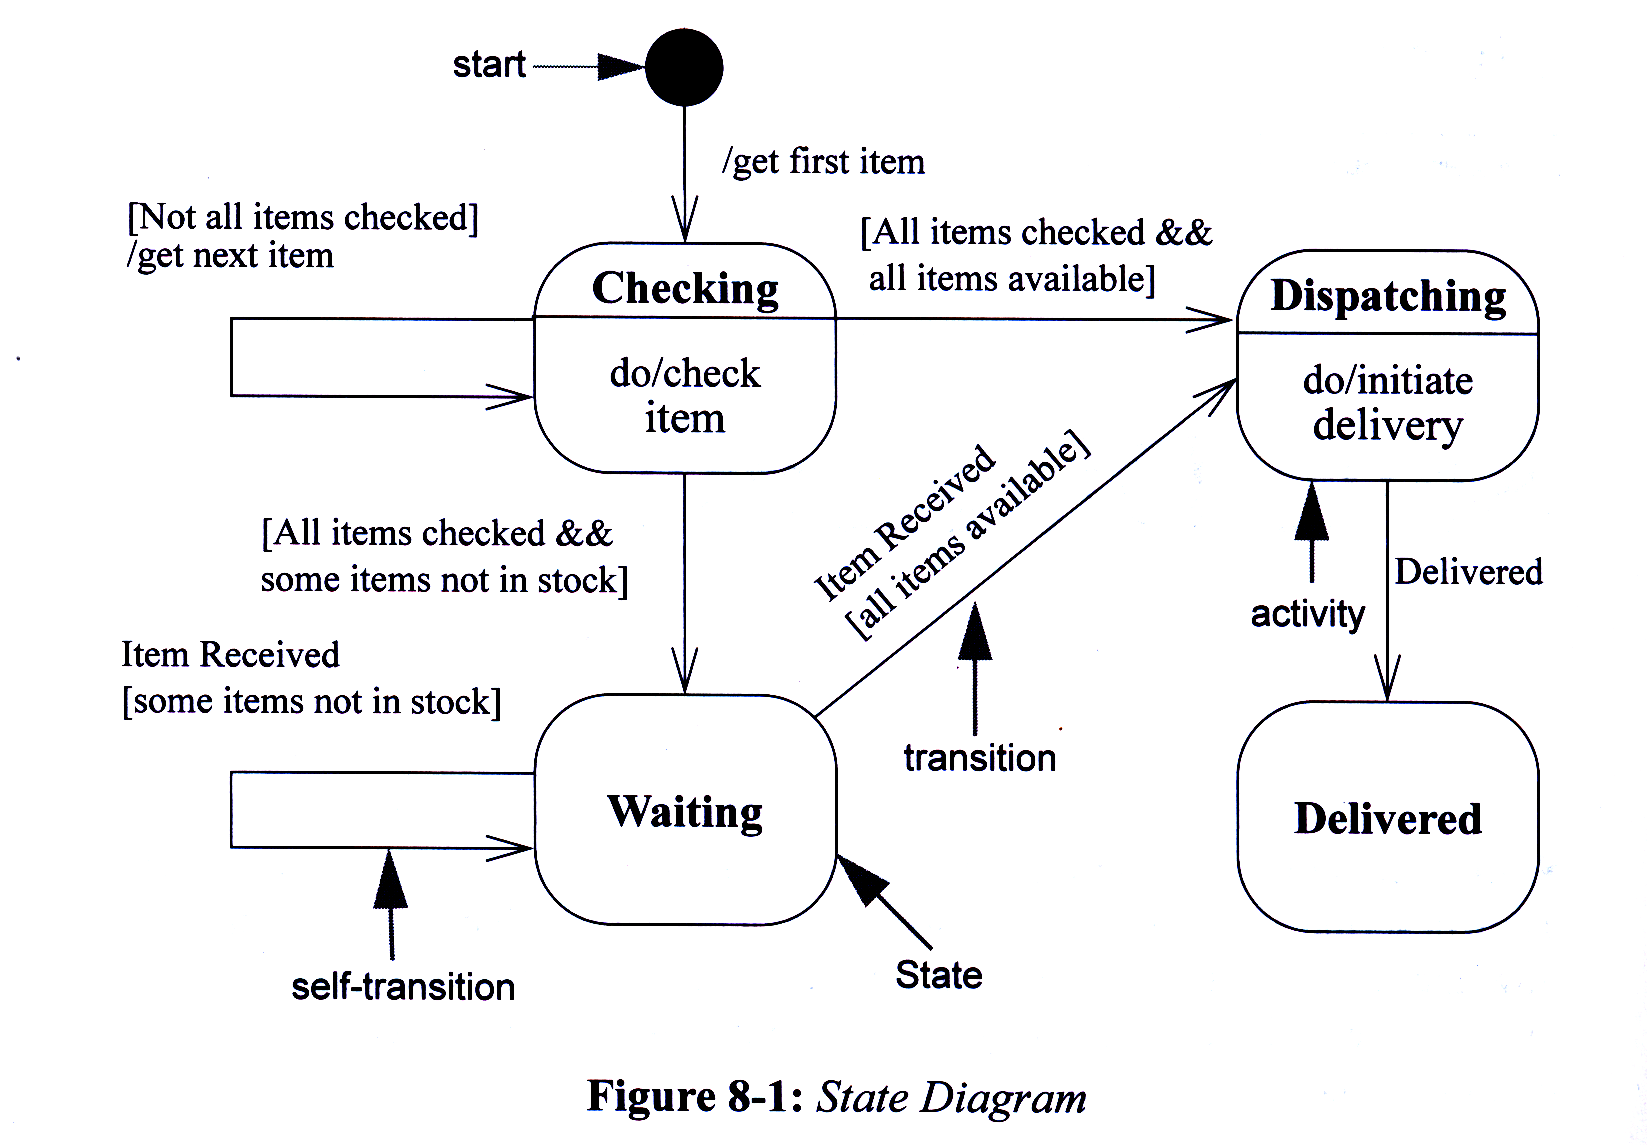
\includegraphics[width=0.7\textwidth]{images/statediagram1}
\end{center}

\paragraph{States.} This state diagram illustrates the states of an order 
in an order processing system.  The order object has four states,
represented by boxes, with the name of the state in the upper half of
the box: ``checking'', ``dispatching'', ``waiting'', and ``delivered''.
The lower half explains what the activity in that state is; for
instance, the ``dispatching'' state initiates the delivery of the
order. In ECE155, you can always put ``do'' before the slash
and the activity after the slash.

In general, a state has a name and may have an activity. Objects
carry out activities, and these activities take some amount of time.

\paragraph{Transitions.} 
The edges in the graph represent transitions between states.
Transitions may optionally be labelled. There are three parts
to a transition label, as follows: \emph{Event [Guard] / Action}.
For instance, the self-transition from the ``checking'' state
contains the guard ``[not all items checked]'' and performs
the action ``get next item''. 

An event is something that happens to an object, like ``Item
Received''.  A guard is a logical condition that states the conditions
under which the event may occur (e.g. ``[some items not in stock]'').
Objects carry out actions, e.g. ``get next
item''; actions must occur quickly and be uninterruptible (contrast
this with an activity, which takes longer and gets interrupted by
events).

An object takes a transition if the event occurs and the guard is true.
Before it completes the transition and enters the destination state, it
carries out the action.

UML state machines should be designed to be deterministic: at most one
transition should be activated at once.

\paragraph{Superstates.} State diagrams may get too complicated
to easily understand. UML state diagrams include the notion of
hierarchical nesting to help you write clearer diagrams; such diagrams
allow you to see the higher-level structure of the system.

In particular, UML state diagrams include the notion of a \emph{superstate}.
A superstate may contain nested states and transitions, which make up a
state machine for some subset of the entire machine's behaviour. The following
example includes an example of a superstate, ``active'', which includes the
``checking'' and ``dispatching'' states inside it.

Note also that there are transitions from individual states inside the
superstate, e.g. from ``dispatching'' to ``delivered'', as well as a transition
from the superstate to the ``cancelled'' state. This transition means that
either of the states in the superstate can get to ``cancelled''. It is
equivalent to drawing transitions from both ``dispatching'' and ``checking''
to ``cancelled''.

%\begin{center}
%\includegraphics[width=.6\textwidth,angle=270]{L28-statediagram2.pdf}
%\end{center}
\begin{center}
% Graphic for TeX using PGF
% Title: /home/plam/courses/ece155-s11/lectures/L28-statediagram2.dia
% Creator: Dia v0.97.1
% CreationDate: Sun Jul  3 08:55:14 2011
% For: plam
% \usepackage{tikz}
% The following commands are not supported in PSTricks at present
% We define them conditionally, so when they are implemented,
% this pgf file will use them.
\ifx\du\undefined
  \newlength{\du}
\fi
\setlength{\du}{15\unitlength}
\begin{tikzpicture}
\pgftransformxscale{1.000000}
\pgftransformyscale{-1.000000}
\definecolor{dialinecolor}{rgb}{0.000000, 0.000000, 0.000000}
\pgfsetstrokecolor{dialinecolor}
\definecolor{dialinecolor}{rgb}{1.000000, 1.000000, 1.000000}
\pgfsetfillcolor{dialinecolor}
\pgfsetlinewidth{0.100000\du}
\pgfsetdash{}{0pt}
\pgfsetdash{}{0pt}
\pgfsetmiterjoin
\definecolor{dialinecolor}{rgb}{1.000000, 1.000000, 1.000000}
\pgfsetfillcolor{dialinecolor}
\fill (0.350000\du,3.550000\du)--(0.350000\du,8.650000\du)--(21.150000\du,8.650000\du)--(21.150000\du,3.550000\du)--cycle;
\definecolor{dialinecolor}{rgb}{0.000000, 0.000000, 0.000000}
\pgfsetstrokecolor{dialinecolor}
\draw (0.350000\du,3.550000\du)--(0.350000\du,8.650000\du)--(21.150000\du,8.650000\du)--(21.150000\du,3.550000\du)--cycle;
\pgfsetlinewidth{0.100000\du}
\pgfsetdash{}{0pt}
{\pgfsetcornersarced{\pgfpoint{0.500000\du}{0.500000\du}}\definecolor{dialinecolor}{rgb}{1.000000, 1.000000, 1.000000}
\pgfsetfillcolor{dialinecolor}
\fill (0.800000\du,4.550000\du)--(0.800000\du,7.150000\du)--(6.540000\du,7.150000\du)--(6.540000\du,4.550000\du)--cycle;
}{\pgfsetcornersarced{\pgfpoint{0.500000\du}{0.500000\du}}\definecolor{dialinecolor}{rgb}{0.000000, 0.000000, 0.000000}
\pgfsetstrokecolor{dialinecolor}
\draw (0.800000\du,4.550000\du)--(0.800000\du,7.150000\du)--(6.540000\du,7.150000\du)--(6.540000\du,4.550000\du)--cycle;
}% setfont left to latex
\definecolor{dialinecolor}{rgb}{0.000000, 0.000000, 0.000000}
\pgfsetstrokecolor{dialinecolor}
\node at (3.670000\du,5.645000\du){Checking};
% setfont left to latex
\definecolor{dialinecolor}{rgb}{0.000000, 0.000000, 0.000000}
\pgfsetstrokecolor{dialinecolor}
\node[anchor=west] at (1.300000\du,6.445000\du){do/ check item};
\definecolor{dialinecolor}{rgb}{0.000000, 0.000000, 0.000000}
\pgfsetstrokecolor{dialinecolor}
\draw (0.800000\du,5.850000\du)--(6.540000\du,5.850000\du);
\pgfsetlinewidth{0.100000\du}
\pgfsetdash{}{0pt}
\definecolor{dialinecolor}{rgb}{0.000000, 0.000000, 0.000000}
\pgfsetfillcolor{dialinecolor}
\pgfpathellipse{\pgfpoint{3.650000\du}{0.850000\du}}{\pgfpoint{0.500000\du}{0\du}}{\pgfpoint{0\du}{0.500000\du}}
\pgfusepath{fill}
\pgfsetlinewidth{0.100000\du}
\pgfsetdash{}{0pt}
{\pgfsetcornersarced{\pgfpoint{0.500000\du}{0.500000\du}}\definecolor{dialinecolor}{rgb}{1.000000, 1.000000, 1.000000}
\pgfsetfillcolor{dialinecolor}
\fill (13.500000\du,4.550000\du)--(13.500000\du,7.150000\du)--(20.720000\du,7.150000\du)--(20.720000\du,4.550000\du)--cycle;
}{\pgfsetcornersarced{\pgfpoint{0.500000\du}{0.500000\du}}\definecolor{dialinecolor}{rgb}{0.000000, 0.000000, 0.000000}
\pgfsetstrokecolor{dialinecolor}
\draw (13.500000\du,4.550000\du)--(13.500000\du,7.150000\du)--(20.720000\du,7.150000\du)--(20.720000\du,4.550000\du)--cycle;
}% setfont left to latex
\definecolor{dialinecolor}{rgb}{0.000000, 0.000000, 0.000000}
\pgfsetstrokecolor{dialinecolor}
\node at (17.110000\du,5.645000\du){Dispatching};
% setfont left to latex
\definecolor{dialinecolor}{rgb}{0.000000, 0.000000, 0.000000}
\pgfsetstrokecolor{dialinecolor}
\node[anchor=west] at (14.000000\du,6.445000\du){do/ initiate delivery};
\definecolor{dialinecolor}{rgb}{0.000000, 0.000000, 0.000000}
\pgfsetstrokecolor{dialinecolor}
\draw (13.500000\du,5.850000\du)--(20.720000\du,5.850000\du);
\pgfsetlinewidth{0.100000\du}
\pgfsetdash{}{0pt}
{\pgfsetcornersarced{\pgfpoint{0.500000\du}{0.500000\du}}\definecolor{dialinecolor}{rgb}{1.000000, 1.000000, 1.000000}
\pgfsetfillcolor{dialinecolor}
\fill (15.050000\du,10.825000\du)--(15.050000\du,12.625000\du)--(19.117500\du,12.625000\du)--(19.117500\du,10.825000\du)--cycle;
}{\pgfsetcornersarced{\pgfpoint{0.500000\du}{0.500000\du}}\definecolor{dialinecolor}{rgb}{0.000000, 0.000000, 0.000000}
\pgfsetstrokecolor{dialinecolor}
\draw (15.050000\du,10.825000\du)--(15.050000\du,12.625000\du)--(19.117500\du,12.625000\du)--(19.117500\du,10.825000\du)--cycle;
}% setfont left to latex
\definecolor{dialinecolor}{rgb}{0.000000, 0.000000, 0.000000}
\pgfsetstrokecolor{dialinecolor}
\node at (17.083750\du,11.920000\du){Delivered};
\pgfsetlinewidth{0.100000\du}
\pgfsetdash{}{0pt}
{\pgfsetcornersarced{\pgfpoint{0.500000\du}{0.500000\du}}\definecolor{dialinecolor}{rgb}{1.000000, 1.000000, 1.000000}
\pgfsetfillcolor{dialinecolor}
\fill (1.950000\du,10.825000\du)--(1.950000\du,12.625000\du)--(6.100000\du,12.625000\du)--(6.100000\du,10.825000\du)--cycle;
}{\pgfsetcornersarced{\pgfpoint{0.500000\du}{0.500000\du}}\definecolor{dialinecolor}{rgb}{0.000000, 0.000000, 0.000000}
\pgfsetstrokecolor{dialinecolor}
\draw (1.950000\du,10.825000\du)--(1.950000\du,12.625000\du)--(6.100000\du,12.625000\du)--(6.100000\du,10.825000\du)--cycle;
}% setfont left to latex
\definecolor{dialinecolor}{rgb}{0.000000, 0.000000, 0.000000}
\pgfsetstrokecolor{dialinecolor}
\node at (4.025000\du,11.920000\du){Cancelled};
% setfont left to latex
\definecolor{dialinecolor}{rgb}{0.000000, 0.000000, 0.000000}
\pgfsetstrokecolor{dialinecolor}
\node[anchor=west] at (9.700000\du,4.250000\du){Active};
\pgfsetlinewidth{0.100000\du}
\pgfsetbuttcap
\pgfsetdash{}{0pt}
{
\definecolor{dialinecolor}{rgb}{0.000000, 0.000000, 0.000000}
\pgfsetfillcolor{dialinecolor}
% was here!!!
\pgfsetarrowsend{to}
\definecolor{dialinecolor}{rgb}{0.000000, 0.000000, 0.000000}
\pgfsetstrokecolor{dialinecolor}
\draw (6.540000\du,5.850000\du)--(10.020000\du,5.850000\du)--(10.020000\du,5.850000\du)--(13.500000\du,5.850000\du);
}
% setfont left to latex
\definecolor{dialinecolor}{rgb}{0.000000, 0.000000, 0.000000}
\pgfsetstrokecolor{dialinecolor}
\node at (10.050000\du,6.600000\du){\ensuremath{[}all items available\ensuremath{]}};
\pgfsetlinewidth{0.100000\du}
\pgfsetbuttcap
\pgfsetdash{}{0pt}
{
\definecolor{dialinecolor}{rgb}{0.000000, 0.000000, 0.000000}
\pgfsetfillcolor{dialinecolor}
% was here!!!
\pgfsetarrowsend{to}
\definecolor{dialinecolor}{rgb}{0.000000, 0.000000, 0.000000}
\pgfsetstrokecolor{dialinecolor}
\draw (3.650000\du,1.350000\du)--(3.650000\du,2.950000\du)--(3.670000\du,2.950000\du)--(3.670000\du,4.550000\du);
}
% setfont left to latex
\pgfsetlinewidth{0.100000\du}
\pgfsetbuttcap
\pgfsetdash{}{0pt}
{
\definecolor{dialinecolor}{rgb}{0.000000, 0.000000, 0.000000}
\pgfsetfillcolor{dialinecolor}
% was here!!!
\pgfsetarrowsend{to}
\definecolor{dialinecolor}{rgb}{0.000000, 0.000000, 0.000000}
\pgfsetstrokecolor{dialinecolor}
\draw (17.110000\du,7.150000\du)--(17.110000\du,8.987500\du)--(17.083750\du,8.987500\du)--(17.083750\du,10.825000\du);
}
% setfont left to latex
\pgfsetlinewidth{0.100000\du}
\pgfsetbuttcap
\pgfsetdash{}{0pt}
{
\definecolor{dialinecolor}{rgb}{0.000000, 0.000000, 0.000000}
\pgfsetfillcolor{dialinecolor}
% was here!!!
\pgfsetarrowsend{to}
\definecolor{dialinecolor}{rgb}{0.000000, 0.000000, 0.000000}
\pgfsetstrokecolor{dialinecolor}
\draw (10.750000\du,8.650000\du)--(10.750000\du,9.737500\du)--(4.025000\du,9.737500\du)--(4.025000\du,10.825000\du);
}
% setfont left to latex
\end{tikzpicture}


(From: \url{http://atlas.kennesaw.edu/~dbraun/csis4650/A&D/UML_tutorial/state.htm}. Accessed July 3, 2011.)
\end{center}

\paragraph{Timing.} Timing is important for embedded systems.
Your documentation should explain what ``quickly'' (as in an action)
means; UML doesn't say, and it depends on the system.  You can also
write an event that happens after some time, e.g. ``after (20
minutes)''. 

\section*{UML Use Case Diagrams}
The next kind of UML diagram we'll talk about is the use case diagram.
We'll talk about use cases shortly; a use case describes a user's
interaction with the system. In these diagrams, users (or other systems) 
are known as
\emph{actors}, who play roles in the behaviour of the system.  The
following figure from the {\tt embarcadero} site explains:

\begin{center}
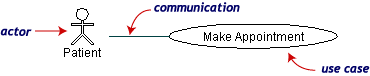
\includegraphics[width=.5\textwidth]{images/usecase-explanation.png}
\end{center}

Here is a case with multiple actors:

\begin{center}
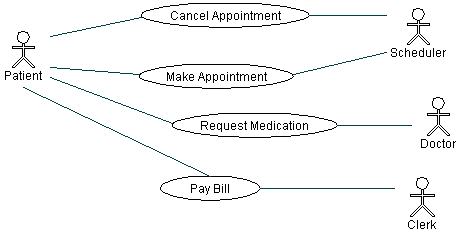
\includegraphics[width=.45\textwidth]{images/usecase-multiple.png}
\end{center}
It's just a coincidence that each use case has two actors.

Finally, here's another use case diagram,
from \url{http://msdn.microsoft.com/en-us/library/dd409427%28VS.100%29.aspx}
(accessed March 10, 2011).

\begin{center}
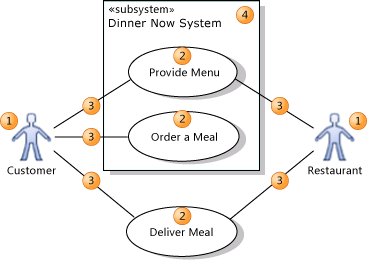
\includegraphics[width=.3\textwidth]{images/dinnernow.png}
\end{center}

Again, we have 1) actors, 2) use cases, 3) communication, and, new to this
figure, 4) subsystems or components. 


The following diagram indicates
relationships between use cases and actors.

\begin{center}
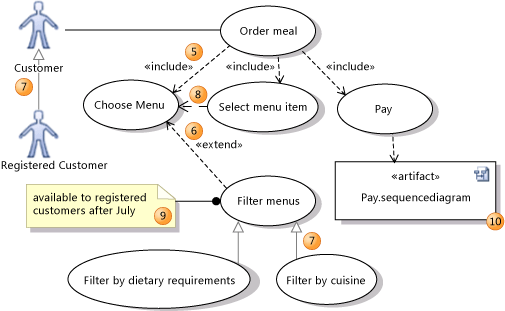
\includegraphics[width=.55\textwidth]{images/dinnernow2.png}
\end{center}

Here we have 5) inclusion stereotypes on dependencies; 6) extension
stereotypes on dependencies; 7) inheritance relationships between use cases;
8) plain dependencies; 9) comments; and 10) references to other artifacts.

\begin{itemize}
\item A \emph{communication} (solid line) represents a relationship
between an actor and a use case.
\item An \emph{inclusion} (dashed line, \guillemotleft include \guillemotright stereotype)
represents an invocation relationship between use cases; the first use 
case must call the second one.
\item An \emph{extension} (dashed line, \guillemotleft extend \guillemotright stereotype)
represents an optional invocation of a use case.
\item A \emph{generalization} or \emph{specialization} represents
a case where an actor or use case inherits from another actor or use case.
\end{itemize}

\paragraph{Why use UML Use Case Diagrams?} These diagrams can be
useful for 1) documenting essential features (requirements) of
a software system; 2) communicating system behaviour to clients; 3)
generating appropriate test cases for scenarios.

\section*{UML Sequence Diagrams}
The last kind of UML diagram we'll talk about is the sequence
diagram. UML sequence diagrams express system behaviour as a sequence
of events and activities. (Message sequence charts do the same thing.)
In a sequence diagram, you'll find objects, lifelines, messages,
action boxes, and gates.

\begin{itemize}
\item \emph{Instances} of objects are shown as boxes at the top of the diagram.
\item \emph{Lifelines} are shown as vertical dashed lines, extending
downwards from instances of the objects, to denote the passing of time.
\item \emph{Messages}, drawn as horizontal lines, denote the
communication of events between objects.
\item \emph{Action boxes}, drawn as boxes on top of lifelines, denote
the occurrence of activities.
\item \emph{Gates}, shown as filled circles on the boundary of the diagram,
denote the occurrence of an external event.
\end{itemize}

\paragraph{Example 1.} Consider the following sequence diagram from
a financial reporting system. (IBM, \emph{UML basics: The sequence
  diagram},
\url{http://www.ibm.com/developerworks/rational/library/3101.html},
accessed March 10, 2011).

\begin{center}
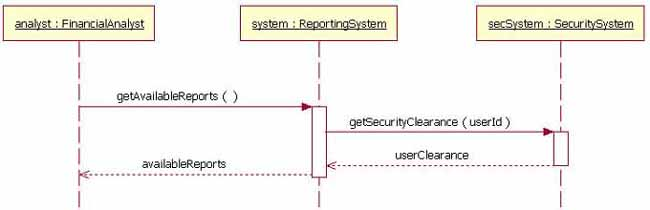
\includegraphics[width=0.7\textwidth]{images/uml_sequence.png}
\end{center}
Solid lines are initiating messages, while dashed lines are responses.
We can also see synchronous messages (solid arrowhead---all initiating
messages in the above example) and asynchronous messages (stick
arrowhead---responses).

There are more elements that you can put in UML sequence diagrams,
including actors (indicating interactions between the system and
its users); destroy elements (indicating the end of an object
instance); scenario elements (denoting a set of alternative actions);
and timer elements (for discussing timed events). You can find
more information about those elements at \url{http://www.sequencediagrameditor.com/uml/sequence-diagram.htm}.

\paragraph{Example 2.} Here is another sequence diagram, again from the
\emph{UML Basics} site.
\begin{center}
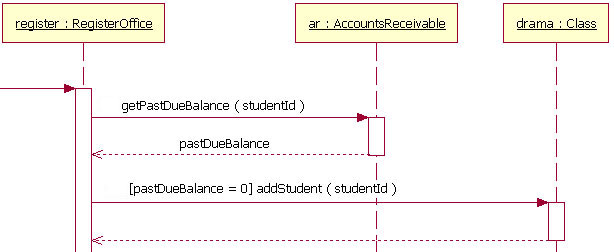
\includegraphics[width=0.7\textwidth]{images/student_records.png}
\end{center}
We can note guards on the messages, which need to be satisfied before
the message gets sent.

\paragraph{When to use Sequence Diagrams.} UML sequence
diagrams help document messages going between different instances of
objects, including the ordering in which these events occur, if
applicable (for synchronous events).

You need to exercise judgment to include the right level of detail;
as in any model, too much detail makes the model difficult to
understand, and too little detail doesn't document anything. You
can use more than one UML sequence diagram to document a large system.



\bibliographystyle{alpha}
\bibliography{155}


\end{document}